\chapter{Introduction}

\section{The problem and motivation}

Starting a new module is never as easy as just logging onto the current VLE (Virtual Learning Environment), selecting a module and knowing exactly where the resources will be and how to access them. With each module, there comes a new learning curve of how to access the learning materials and interact with the tutor. 

Cardiff University currently uses a VLE called Blackboard Learn (also known as Learning Central), which allows tutors to customise their modules in a large number of ways. This is useful for tutors, giving them the freedom to upload and set up the layout of their modules the way they wish. With this level of freedom, each tutor can decide to setup up their online module layout very differently from the next tutor. Every tutor has their own idea as to how students should be taught and how they should receive the resources they provide. They are able to do what they believe is best for their students, with the freedom to change, add and withhold sections. This freedom allows them to experiment with different ways of delivering their course without being locked into one way of doing things.

However, despite the advantages that come with this amount of flexibility in the system, there are downsides for the students. When students start a new module, they must learn to navigate many different layouts, often during the same semester and even within the same module. Some tutors add all the resources into one long stream of content,

\begin{figure}[H]
    \centering
    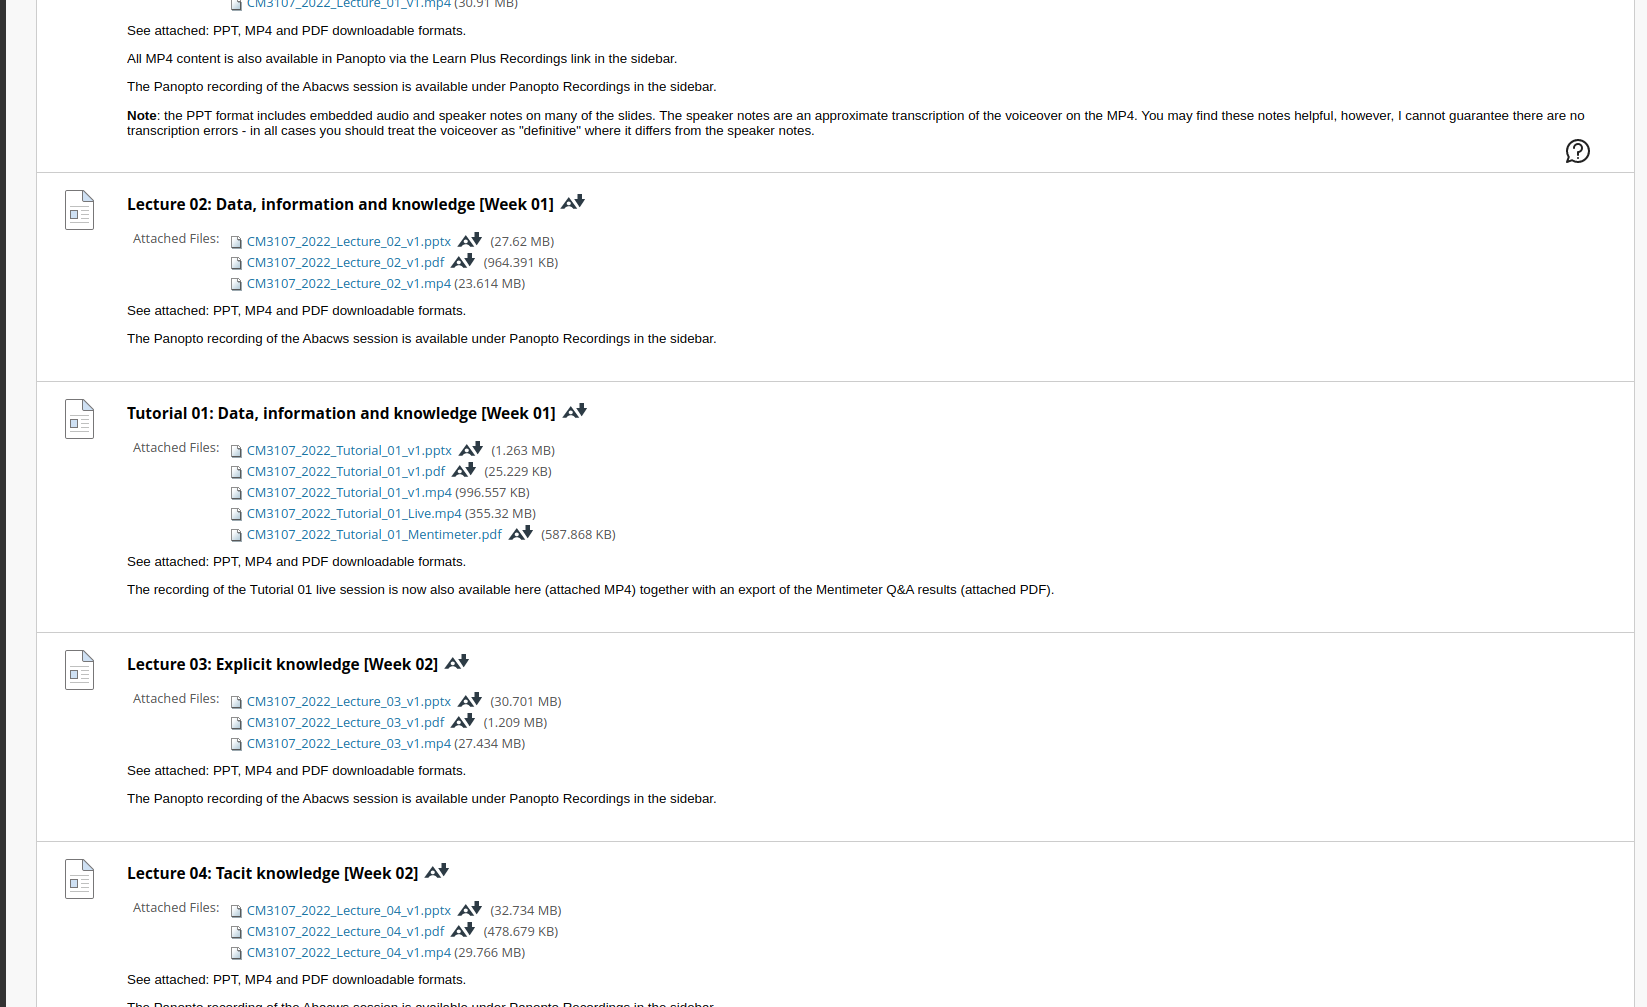
\includegraphics[scale=0.20]{images/LC screenshots/LC module without folders.png}
    \caption{LC module without folders}
    \label{fig:my_label}
\end{figure}

some separate each week into different folders, 

\begin{figure}[H]
    \centering
    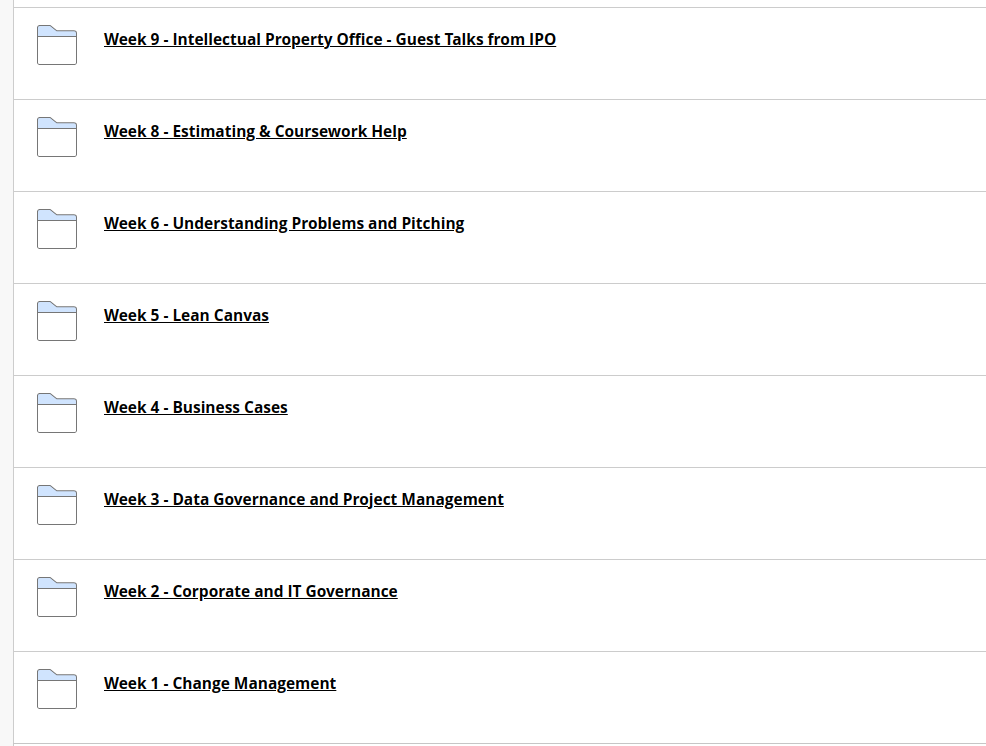
\includegraphics[scale=0.25]{images/LC screenshots/LC module with folders.png}
    \caption{LC module with folders}
    \label{fig:my_label}
\end{figure}

some add different folders for each tutor, 

\begin{figure}[H]
    \centering
    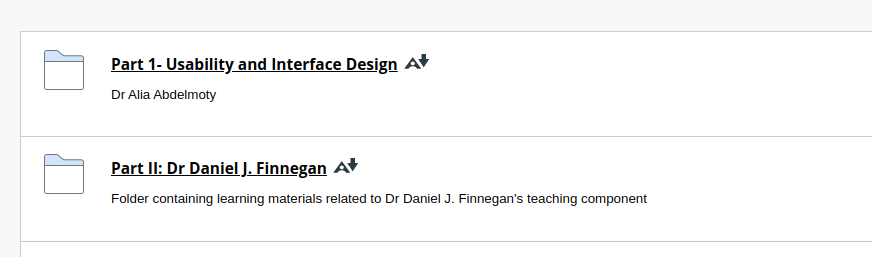
\includegraphics[scale=0.25]{images/LC screenshots/LC module with folders diff tutors.png}
    \caption{LC module with different folders for different tutors}
    \label{fig:my_label}
\end{figure}

and some use a combination of different organisation techniques.

\begin{figure}[H]
    \centering
    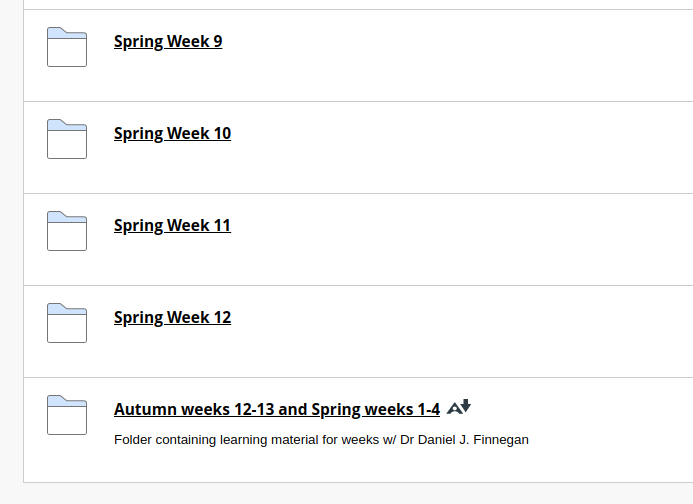
\includegraphics[scale=0.25]{images/LC screenshots/LC module with folders diff combo.png}
    \caption{LC module with a combination of different folder organisation types}
    \label{fig:my_label}
\end{figure} 

Three main applications are also used to provide online lectures: Microsoft Teams, Zoom and Blackboard. As there is no standard university-wide or across-the-school (School of Computer Science), tutors are left to decide on which tool they want to use. Even within the same module, tutors seem not to be to decide on which video conferencing tool to use. For one module in first year, we had three different tutors, and each tutor used an application. The result of this is that each module's content, structure and delivery can vary widely from one module to the next, creating a lack of consistency. This can ultimately leave students confused, forgetting which tutor used what application and not being able to find where they posted about the one they plan on using.

\section{The why}

From over two years of using Learning Central (LC) it has become very irritating having to re-figure out the structure of each tutor's setup, how they prefer to be contacted and conduct their lectures. If students are required to learn a new way of interacting with each online version of a module every time, this could impact how well they are able to learn, especially in the initial stage of the module. Students have a hard enough time trying to balance 60 hours a week studying, a social life and general day-to-day task, with many needing to add work on top of that just to afford to live. If there was a single destination to find everything they need to get on with learning in a friendly, structured way, it could improve the experience. It would take away unnecessary mental strain that could be avoided with some kind of standardization.

\section{The aim}

This dissertation aims to create a prototype of an application that combines the functionality of sharing information, resources and asking questions relating to a university module. It is also combined with a real-time chatting system for users to both socialise and discuss module-related content. The application is designed to be a consistent experience regardless of which module the user is taking. The aim is not to create a perfect, award-winning solution first time, where modules are laid out perfectly for every tutor and student. The prototype is designed to be a starting point and to be developed further into a start-up, becoming the MVP (Minimal Viable Product) and, with some hope, much more.

The application is built to show a proof of concept with as much functionality as possible, which can be added by one person in a short amount of time. The idea is to aim to use the best software development practices but keeping in mind that it is built quickly and dirty as not to waste too much time with perfect code, as the  concept may not work. As this is designed to be an MVP, developing into a startup, the application needs to have enough functionality to determine if users would be willing to use it. A better version would be developed at a later stage as it starts to grow.